%!TEX root = tesis.tex
\chapter{Aprendizaje en un \ssolver paralelo y distribuido}
\label{aprendizaje-pardist}

En el Cap.~\ref{ssolver-pardist} vimos que el enfoque de distribución aplicado
consigue disminuir el tiempo necesario para resolver una serie de problemas de
tamaño considerable. Al mismo tiempo observamos que existen casos en los que
la eficiencia --entendida como cuánto ganamos por cada unidad de \hard
agregada al cómputo de un problema-- resulta pobre. Planteamos como conjetura
que esta situación se debe, en gran medida, a una importante cantidad de
retrabajo que se produce como consecuencia del particionado de un problema en
diversos subproblemas. Nuestra hipótesis es que la reutilización de cláusulas
aprendidas puede ayudar a disminuir la cantidad de retrabajo que se produce
como efecto del particionado.

La existencia de retrabajo se evidencia en que si bien al partir un problema
en subproblemas, el subproblema más grande suele ser más chico que el padre,
la suma del tiempo requerido para resolver todos los subproblemas hijos es
considerablemente mayor que el tiempo requerido para resolver el problema
padre. Debido al esquema de particionado recursivo, este incremento en el
tiempo total de cómputo requerido para resolver un problema se vuelve
sustancial.

En el presente capítulo desarrollaremos un mecanismo de reutilización del
conocimiento adquirido durante la ejecución de cada subproblema. Este
mecanismo persigue dos objetivos principales: verificar la hipótesis planteada
y, de ser posible,  disminuir los tiempos requeridos para resolver un problema
aumentando la eficiencia de la herramienta.

\section{Justificación del enfoque}

El enfoque de particionamiento recursivo, basado en \emph{guiding paths}, que
hemos adoptado para la construcción de la herramienta también influye en la
elección de un mecanismo adecuado para compartir información de cláusulas
aprendidas. 

\newcommand{\roottask}{\ensuremath{<\varphi_R, \emptyset>}\xspace}
\newcommand{\task}{\ensuremath{<\varphi, \emptyset>}\xspace}
\newcommand{\nonemptytask}{\ensuremath{<\varphi, C>}\xspace}

Consideremos ahora que un problema no es ya únicamente una fórmula $\varphi$
sino una tupla $<\varphi, C>$ donde $C$ es un conjunto de cláusulas tales que
$(\forall v) (v \models \varphi \Longleftrightarrow v \models \varphi
\bigwedge C)$ llamado conjunto de cláusulas aprendidas. En este contexto el
problema original es la tupla \roottask donde $\varphi_R$ denota la fórmula
original que se desea verificar. En este modelo, al partir un problema \task
levantando (por ejemplo) la variable $u$ obtenemos dos nuevos subproblemas
$<\varphi_u, \emptyset>$ y $<\varphi_{-u}, \emptyset>$. 

Notemos entonces que dado un problema \nonemptytask podemos generar los
subproblemas que resultan de levantar la variable $u$ como sigue:
$t_u=<\varphi_u, C_u>$ y $t_{-u}=<\varphi_{-u}, C_{-u}>$ (donde $C_u$ es el
conjunto de cláusulas que resulta de reemplazar las apariciones de la variable
$u$ por el valor $1$ en el conjunto $C$ y $C_{-u}$ es el resultado de
reemplazar las apariciones de la variable $u$ por el valor $0$) sin alterar la
corrección de la herramienta. Esto se debe a que si $v \models \varphi_u$
entonces $v\cup\{u\leftarrow1\} \models \varphi$ y por lo tanto
$v\cup\{u\leftarrow1\} \models \varphi \bigwedge C$ de lo que se deduce que $v
\models \varphi_u \bigwedge C_u$. Lo mismo vale para el caso $\varphi_{-u}$.

Más aún, lo antedicho vale también para cualquier subconjunto de $C$. Esto
induce una manera \emph{natural} de reutilización de las cláusulas aprendidas
que llamaremos \emph{herencia}. Este mecanismo consiste en que, al generar
nuevos subproblemas a partir de un problema padre \nonemptytask, los
subproblemas hijos son generados con un subconjunto de $C$ como conjunto de
cláusulas aprendidas. Llamaremos \emph{criterio} a cada forma distinta de
obtener un subconjunto de un conjunto de cláusulas $C$.


\subsubsection{Consideraciones de escalabilidad}

Más allá de la naturalidad del enfoque inducido por el esquema de
particionado, nos interesa también evitar cualquier método que introduzca
nuevos cuellos de botella en la arquitectura. Por ejemplo, no sería aceptable
la incorporación de una gran base de datos centralizada en la que todos los
\ws almacenen las cláusulas que van aprendiendo y que todos los \ws deban
consultar.

Tampoco sería aceptable un grafo completo de comunicación permanente para
lograr ese mismo fin, es decir, hacer que cada \w le comunique (o consulte) a
todos los demás las cláusulas que va(n) aprendiendo.


\subsubsection{Independencia del \ssolver particular utilizado}

Por otro lado, como ya hemos señalado en el Cap.~\ref{ssolver-pardist}, nos
interesa que el \ssolver secuencial que utiliza cada uno de los \ws sea fácil
de actualizar y/o de reemplazar por otro componente \ots similar. Si bien
suelen ser necesarios algunos cambios para lograr que un \ssolver permita la
inyección \emph{inicial} de cláusulas aprendidas (en lugar de comenzar sin
ninguna), por lo general tales cambios se reducen a cuestiones de interfaz y
no revisten mayor dificultad.

Es más ambicioso, en cambio, pretender poder inyectar nuevas cláusulas
aprendidas en cualquier momento \emph{durante} el proceso de búsqueda. Para
ello habría que introducir modificaciones mucho más fuertemente acopladas a la
versión particular de \ssolver en uso, sus algoritmos, estructuras de datos e
invariantes particulares.

\

Es por estos factores que optamos por implementar un esquema de reutilización
de cláusulas aprendidas basado en herencia. En esencia el esquema funciona de
acuerdo a lo detallado al comienzo de esta sección. En particular, a la hora
de partir un problema en nuevos subproblemas un \emph{criterio} es aplicado al
conjunto de cláusulas aprendidas que el problema padre poseía al momento de
ser abortado. De esta manera se generan los subconjuntos de cláusulas
aprendidas que los subproblemas hijos deberán incorporar antes de comenzar el
análisis. Cabe destacar que si bien la herramienta permite seleccionar un
nuevo criterio de aprendizaje cada vez que un problema es partido, en la
evaluación realizada no se utilizó esta característica sino que se mantuvo un
mismo criterio para toda la corrida.


\subsubsection{Sobre los criterios}
\label{sec:aboutcriteria}

En principio podríamos preguntarnos de dónde surge la necesidad de tener
criterios para la herencia de cláusulas aprendidas. O lo que es lo mismo, por
qué no heredar todas las cláusulas aprendidas del padre. Existen varias
razones que motivan la necesidad de introducir criterios de selección de
cláusulas.

En primer lugar la incorporación de cláusulas aprendidas a un problema
incrementa la cantidad de cláusulas sobre las que es necesario propagar las
decisiones. Esto provoca una ralentización del proceso de propagación que
puede resultar en una disminución del rendimiento del \ssolver secuencial.
Como ya se mencionó en \ref{sec:pruning}, es sabido que incrementar en demasía
la base de datos de cláusulas aprendidas en un \ssolver secuencial se torna
contraproducente. Es por esto que todos los \ssolvers \CDCL secuenciales
cuentan con políticas de recorte de dicha base de datos y que, por lo general,
estas políticas son bastante agresivas.

Otro factor que aboga en contra de mantener la totalidad de las cláusulas
aprendidas por el padre es el hecho de que los subproblemas generados suelen
ser más chicos que el padre. Incluso es bastante común que una buena
proporción de los subproblemas generados al partir un problema padre sean
considerablemente más chicos. En todos estos casos la incorporación de un
conjunto de cláusulas aprendidas extremadamente grande, resultará
inmediatamente contraproducente debido a lo expuesto en el párrafo anterior.

El último motivo para la introducción de criterios de selección es que los
subproblemas generados no son resueltos inmediatamente sino que pasan a formar
parte de la cola de tareas pendientes. Dado que el conjunto de cláusulas
aprendidas de un problema es potencialmente muy grande, heredar la totalidad
de las mismas en cada uno de los subproblemas hijos nos obligaría a pagar un
alto costo debido a la escritura y posterior lectura --hacia y desde memoria
secundaria-- de cada uno de estos conjuntos (potencialmente muy grandes) más
el costo de la posible transmisión por medio de la red. Esto atentaría
directamente contra el desempeño de nuestra herramienta, incrementando en
demasía los costos \emph{fijos} asociados al enfoque.

% Que cada hijo herede TODAS las cláusulas aprendidas por su padre probablemente sea demasiado / contraproducente:
% \begin{itemize}
% \item Por algo los solvers secuenciales van purgando: es sabido que zarparse no es bueno.
% \item OK, el padre sí llegó a todo eso, pero por algo los solvers secuenciales van subiendo de a poco el máximo de aprendidas: es sabido que zarparse desde el primer momento no es buena idea. Y estamos suponiendo que los subproblemas serán más chicos/fáciles que su problema padre.
% \item Y además, la herencia no es inmediata sino mediata. Jugarse a heredar todo implica jugarse a pagar el precio de bajar todo eso a disco, guardar todo eso en storage/pending, leer todo eso de disco, etc. Bocha overhead.
% \end{itemize}

% Por lo tanto vamos a necesitar criterios de selección, subconjunto, etc.


\section{Prueba de concepto}

Con el objetivo de evaluar la pertinencia y viabilidad del enfoque propuesto
para el aprendizaje, llevamos a cabo una prueba de concepto. La misma
consistió en la ejecución de distintos problemas realizando una única
partición y aplicando distintos criterios de selección de cláusulas aprendidas
y comparando los tiempos obtenidos. Para ello cada problema fue ejecutado
durante 60 segundos y luego partido levantando 5 variables para obtener 32
subproblemas. Cada uno de los subproblemas fue ejecutado hasta su
finalización. Dado que, como ya mencionamos, la elección de variables a
levantar influye fuertemente en la distribución de dificultades de los
subproblemas resultantes, cada criterio fue testeado utilizando 10 secuencias
de variables distintas generadas pseudoaleatoriamente. Luego se compararon
tanto los tiempos totales de cómputo invertidos en resolver el problema como
el tiempo del camino crítico (determinado por el subproblema que más tiempo
tomó).


\subsubsection{Resultados obtenidos}

A continuación presentamos los resultados obtenidos en la realización de la
prueba de concepto. Las Fig.~\ref{perchap8}~a~\ref{perchasound8}  se organizan
de la siguiente manera. Cada figura corresponde a la ejecución de distintos
criterios de selección de cláusulas para un problema particular. Cada par de
columnas denotadas con un número decimal corresponde a los resultados
obtenidos con uno de los órdenes pseudoaleatorios. La columna de la izquierda
de cada par de columnas indica el tiempo en segundos requerido para resolver
el camino crítico. Mientras tanto la columna de la derecha indica la sumatoria
del total de tiempos requerido para resolver todos los subproblemas. A su vez,
el último par de columnas de cada figura, denotado con la leyenda ``AVERAGE'',
contiene los promedios de los tiempos obtenidos.

No nos interesaba en esta etapa evaluar cuál o cuáles de los criterios eran
mejores. Por lo tanto obviamos la denominación de los mismos en esta
presentación. Sin embargo es importante aclarar que la última fila contiene
los tiempos obtenidos para el criterio nulo, es decir aquel criterio que
devuelve siempre el conjunto vacío.

El coloreo de las tablas se realizó utilizando una escala desde el color
amarillo hacia el rojo para aquellos criterios que requirieron más tiempo que
el criterio nulo, mientras que se usó una escala del amarillo hacia el verde
para los que requirieron menos tiempo. La escala hacia el color rojo se saturó
en dos veces el tiempo requerido por el criterio nulo mientras que la escala
hacia el verde se saturó en $0.5$ veces el tiempo requerido por el criterio nulo.

\begin{figure}
	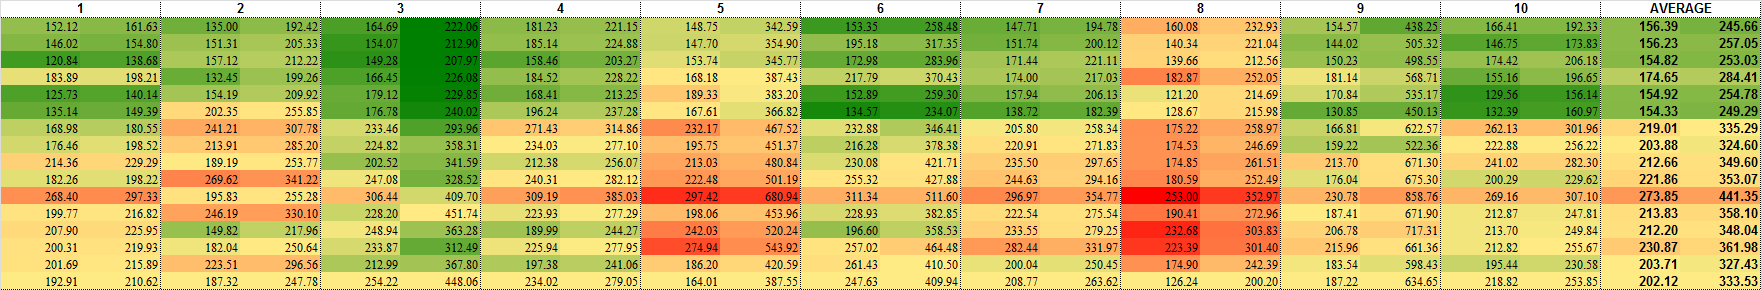
\includegraphics[width=\textwidth]{resultados/p8_percha.png}
	\caption{Routing \emph{scope} 8}
	\label{perchap8}
\end{figure}

\begin{figure}
	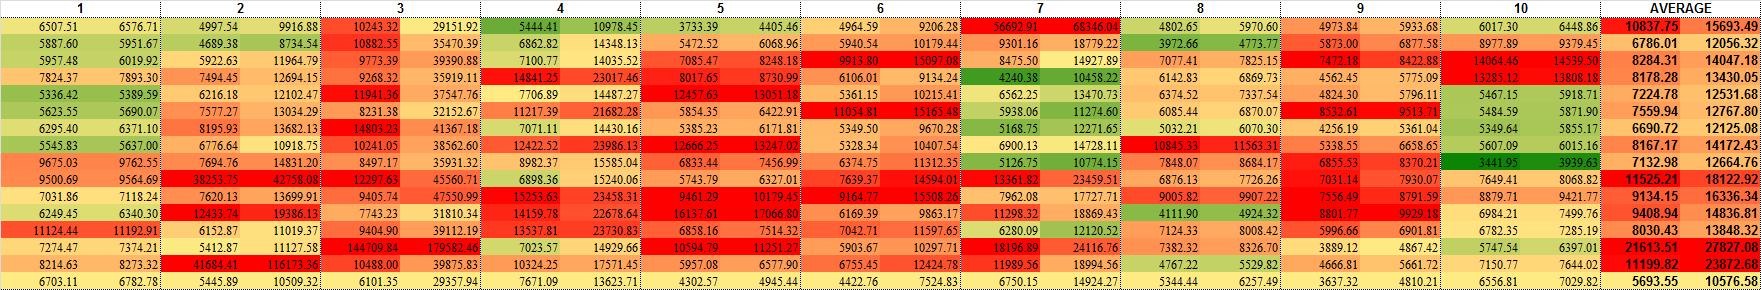
\includegraphics[width=\textwidth]{resultados/p9_percha.png}
	\caption{Routing \emph{scope} 9}
\end{figure}

\begin{figure}
	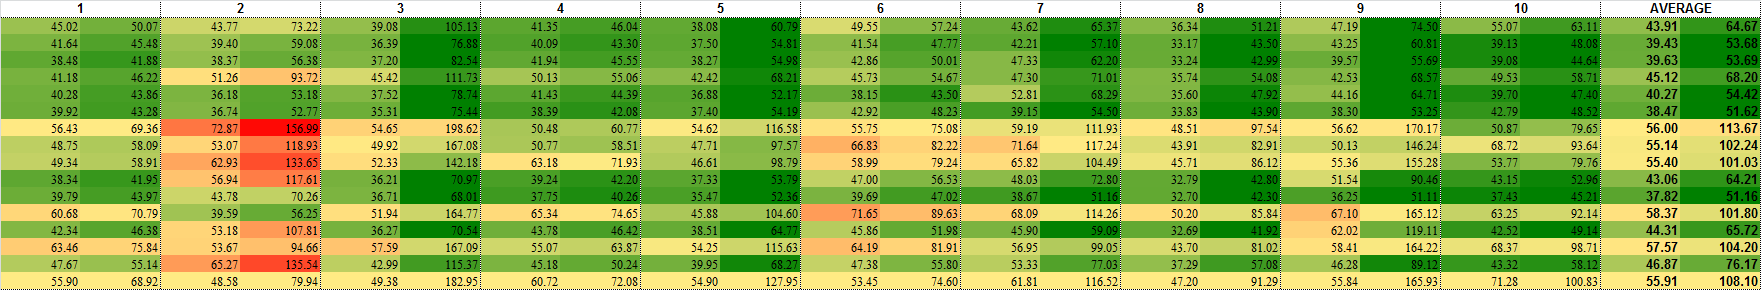
\includegraphics[width=\textwidth]{resultados/k9_percha.png}
	\caption{Closure \emph{scope} 9}
\end{figure}

\begin{figure}
	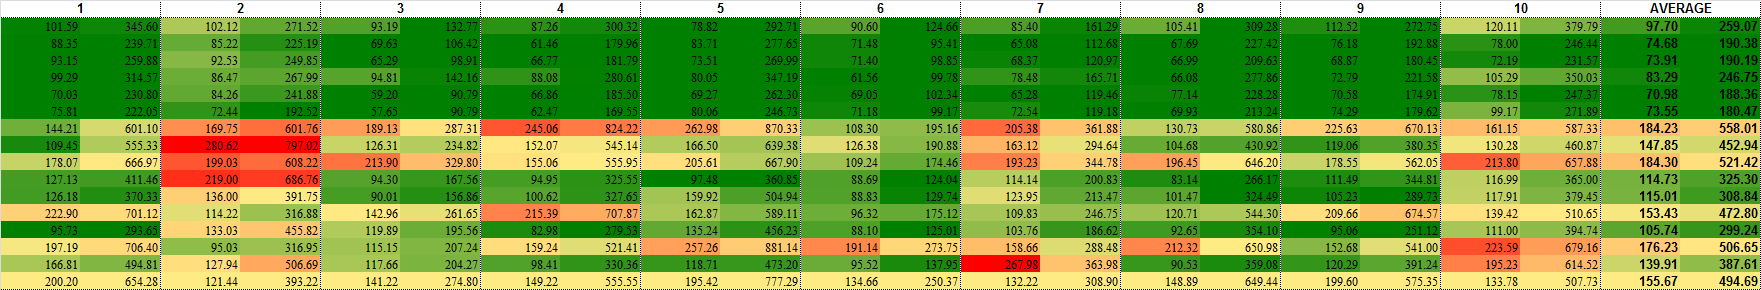
\includegraphics[width=\textwidth]{resultados/k10_percha.png}
	\caption{Closure \emph{scope} 10}
\end{figure}

\begin{figure}
	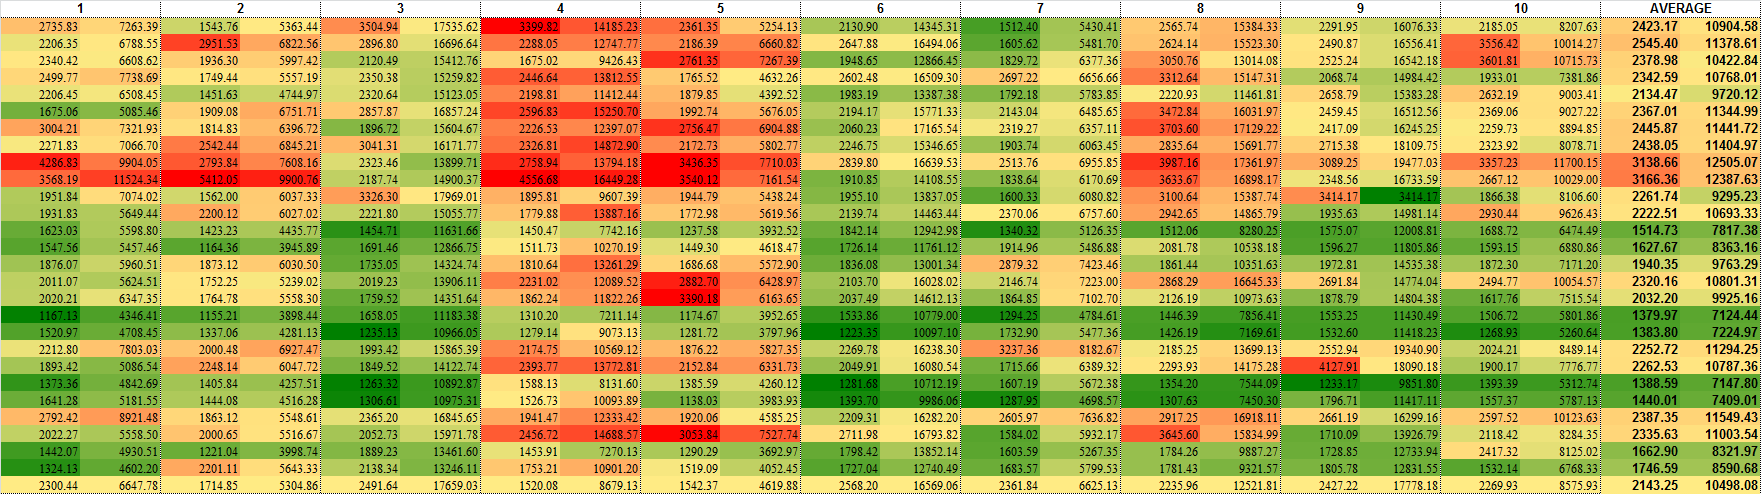
\includegraphics[width=\textwidth]{resultados/soundness8_percha.png}
	\caption{Soundness2 \emph{scope} 8}
	\label{perchasound8}
\end{figure}

Como puede observarse en las figuras, los resultados obtenidos varían
fuertemente de uno a otro problema y en función de cada elección particular de
variables. Además, los resultados no podrían ser del todo concluyentes en
tanto constituyen una aproximación de orden 1 al enfoque \emph{divide-and-
conquer}: en esta prueba de concepto, el problema no se parte recursivamente
sino una única vez en subproblemas.

Más allá de estas limitaciones, cabe observar que en algunos casos varios de
los criterios reportan ganancias considerables. Aún más importante es el hecho
de que para la mayoría de los problemas hay al menos un criterio que reporta
resultados positivos. Interpretamos esto como evidencia suficientemente
alentadora para embarcarnos en una evaluación más realista de la técnica
en el marco de nuestra herramienta distribuida.

\section{Resultados experimentales}

En esta sección mostraremos los resultados experimentales obtenidos a partir
de la implementación de la herencia de cláusulas aprendidas.

Comenzaremos por definir los criterios de selección de cláusulas utilizados.
Cabe aclarar que de aquí en más se considerará que una cláusula aprendida
contiene al menos $2$ literales. Llamaremos \emph{hechos} a las cláusulas de
tamaño $1$.

\subsection{Criterios de selección de cláusulas}

Se probaron tres tipos de criterios:

\begin{itemize}
	\item Por tamaño: Este criterio refiere a la cantidad de literales intervinientes en una cláusula. La motivación de este criterio surge de la observación de que, cuanto más pequeña sea una cláusula, mayor será la porción del árbol de búsqueda que recorte. Recordemos que, en el contexto de nuestro problema, las cláusulas son disyunciones. Por lo tanto una cláusula que contiene $n$ literales nos evita recorrer una $\frac{1}{2^n}$ parte del espacio de búsqueda. Esto se debe a que, de las $2^n$ valuaciones posibles restringidas a los $n$ literales intervinientes, hay una de ellas --en particular aquella que hace que dicha cláusula sea falsa-- que es descartada gracias a la existencia de esta cláusula aprendida. Por lo tanto ninguna valuación que contenga dicha valuación restringida será viable. Por ende, a menor tamaño de cláusula, mayor será el espacio de búsqueda recortado.

	\item Por actividad: En \ref{sec:longactlbd} se explicó a qué nos referimos por actividad de una cláusula. De ello se desprende que la actividad de una cláusula es un indicador de cuántas veces esa cláusula fue (parcialmente) responsable de que ocurra un conflicto. Es de esperar entonces que las cláusulas con mayor actividad sean más relevantes para evitar recorrer ciertas porciones del espacio de de búsqueda.

	\item Por \emph{LBD}: También en \ref{sec:longactlbd} introdujimos la noción de \emph{Literals Block Distance}. Elegimos utilizar esta medida porque se han reportado muy buenos resultados en \ssolvers secuenciales \cite{satchallenge12,satcomp11,satcomp09} utilizando criterios basados en ella.
\end{itemize}

\subsubsection{Parámetros}

En el caso de los criterios por tamaño, los mismos se generaron a partir de un
parámetro que indica el máximo tamaño que puede terner una cláusula para ser
admitida en la herencia. En este caso, todas las cláusulas cuyo tamaño sea
menor o igual que el indicado por el parámetro pasarán a formar parte de la
herencia.

Los criterios por \emph{LBD} funcionan de la misma manera que los basados en
tamaño. En este caso las cláusulas admitidas en la herencia serán aquellas
cuyo \emph{LBD} sea menor o igual al correspondiente parámetro.

Los criterios por actividad se generan a partir de tres parámetros. En primer
lugar un parámetro binario que indica si se desean conservar las cláusulas más
activas o las menos activas. En segundo lugar un parámetro que indica qué
porcentaje de las cláusulas aprendidas del padre se desea conservar y por
último un parámetro binario que indica si, además, se deben conservar todas
aquellas cláusulas aprendidas cuyo tamaño sea 2 (cláusulas binarias).

La incorporación de las cláusulas binarias en los criterios por actividad
surge del hecho de que el \ssolver secuencial utilizado las maneja de manera
particular. Si bien recorta su base de datos de claúsulas aprendidas de
acuerdo a la actividad, nunca descarta las cláusulas binarias.

Además de los tipos de criterios mencionados también se implementó la
posibilidad de heredar los \emph{hechos} aprendidos (o \emph{facts}). La
herencia de los \emph{facts} se implementó de manera tal que pudiera tanto ser
combinada con los distintos tipos de criterios como utilizada de forma
exclusiva como criterio de herencia.




\subsection{Resultados obtenidos}

A continuación presentamos los resultados obtenidos. Los mismos se dividen en
tres aspectos diferentes. 

\subsubsection{Mejora de la eficiencia por problema}

En la Tabla~\ref{tab:mejorlearning} se presenta la comparación entre los
resultados obtenidos con el \ssolver secuencial, los resultados obtenidos por
nuestra herramienta sin herencia de cláusulas aprendidas y los resultados
obtenidos por nuestra herramienta con herencia de cláusulas aprendidas.

Las primeras siete columnas poseen el exacto mismo significado que en la
Tabla~\ref{tab:resultados}. En la columna ``par. walltime w. inher. best crit.'' consignamos
el mejor tiempo obtenido por nuestra herramienta con algún criterio de
selección de cláusulas aprendidas --incluyendo el criterio nulo--.

La columna ``speedup w. inher. best crit.'' representa la mejoría en el tiempo
percibido obtenida por el mejor criterio. La misma es el resultado de la
divisón $$\frac{\text{seq. walltime}}{\text{par. walltime w. inher. best
crit.}}$$ La columna ``efficiency w. inher. best crit.'' es el resultado de la
división $$\frac{\text{speedup w. inher. best crit.}}{\text{\#\ws}}$$ La
columna ``effic. mult.'' es el resultado de la división
$$\frac{\text{efficiency w. inher. best
crit.}}{\text{efficiency without inheritance}}$$

\begin{sidewaystable}
	\small
	\begin{tabular}{lrrrrrrrrrr}
		\toprule
		problem	&			&	reps.	& 	seq.		&  par. walltime	&	speedup				&	efficiency			& par.	walltime				& speedup 							& efficiency			& eff. \\
				&			&	 		& walltime		&  without 			&	without				&	without				& w. inher.	& w. inher. 	& w. inher.	& mult. \\
				&			&	 		& 				& inheritance 		&	 inheritance		&	 inheritance	 	& best crit.	& best crit. 	& best crit.	&  \\
		\cmidrule(r){1-11}
		Routing	&	8		&		7 	& 308.26		&  60.46		& 5.10x		&	0.08 		& 60.46			&	5.10x	& 0.08		& 1.00 \\
		Routing	&	9		&	6 		& 76168.16		&  407.34		& 	186.99x	&	2.92 		& 387.44		& 196.60x	& 3.07		& 1.05 \\
		Routing	&	$^*$10	&	5 		& $>$1209600.00	&  5046.84		&$>$239.67x	&	$>$3.74 	& 3213.59		&$>$376.40x	& $>$5.88	& 1.57 \\
		\cmidrule(r){1-11}
		Closure	&	11		&	14 		& 749.65		&  291.28		&	2.57x	&	0.04 		& 150.30		&  4.99x	& 0.08		& 1.94 \\
		Closure	&	12		&	5 		& 3983.36		&  1914.45		&	2.08x	&	0.03 		& 266.68		& 14.94x	& 0.23		& 7.18 \\
		Closure	&	13		&  5 		& 16261.35		& 	4362.61		&	3.73x	&	0.06 		& 645.44		& 25.19x	& 0.39		& 6.76 \\
		\cmidrule(r){1-11}
		GC Sound.&	9		&	10 		& 217.31		&  200.85		&	1.08x	&	0.02 		& 168.04		& 1.29x		& 0.02		& 1.20 \\
		GC Sound.&	10		&	7 		&  2855.30		&  1376.89		&	2.07x	&	0.03 		& 592.54		& 4.82x		& 0.08		& 2.32 \\
		\cmidrule(r){1-11}
		GC Compl.	& 8		&	7 		& 180.25		&  61.50		&	2.93x	&	0.05 		& 36.43			& 4.95x		& 0.08		& 1.69 \\
		GC Compl.	& 9	&	5 		& 18643.06		&  1825.60		&	10.21x	&	0.16 		& 390.48		& 47.74x	& 0.75		& 4.68 \\
		\bottomrule
		\\
		\multicolumn{10}{l}{\begin{tiny}$^*$: Se ejecutó por 14 días sin que el \ssolver secuencial consiga un resultado\end{tiny}}
	\end{tabular}
	\caption{Tiempo de ejecución (en segundos) distribuido sin herencia vs. distribuido con herencia de cláusulas aprendidas}
	\label{tab:mejorlearning}
\end{sidewaystable}

En casi todos los casos se obtuvo una disminución en los tiempos de cómputo
con respecto a la versión sin herencia de cláusulas aprendidas. Se observa una
única excepción, el problema Routing con \emph{scope} 8. En este caso el mejor
tiempo fue el obtenido por el criterio nulo. Es decir por la herramienta sin
herencia de cláusulas.

Se observa también una tendencia a que la mejora obtenida por la incorporación
de herencia de cláusulas crezca considerablemente a medida que crece el tamaño
del problema.

Los resultados aquí expuestos permiten verificar la hipotésis de la cual
partimos: efectivamente la incorporación de herencia de cláusulas aprendidas
permitió mitigar los efectos negativos del retrabajo incrementando la
eficiencia en el uso del \hard disponible.

Sin embargo, en ausencia de un oráculo que permita determinar \emph{a priori}
cuál de los criterios es más conveniente en cada ocasión, la implementación de
herencia de cláusulas aprendidas en una herramienta usable en la práctica
depende de nuestra capacidad para determinar cuál de los criterios es el que
mejor se comporta en el caso promedio. Este problema se ataca en las
siguientes secciones.

\subsubsection{Multiplicadores de \emph{speedup} por cada criterio}
\label{sec:resultadosaprendizaje}

En la Tabla~\ref{tab:rescriterios} mostramos los resultados obtenidos para
cada criterio. Llamaremos \emph{speedup multiplier} a la razón que existe
entre el \emph{speedup} obtenido aplicando herencia de cláusulas aprendidas y
el \emph{speedup} obtenido sin herencia.

La columna ``worst speedup multiplier'' consigna el multiplicador obtenido por
el criterio correspondiente para aquel problema en el que obtuvo el peor
multiplicador. La columna ``best speedup multiplier'' consigna el
multiplicador obtenido por el criterio para aquel problema en el que obtuvo el
mejor multiplicador.

Por último, la columna ``avg speedup multiplier'' consigna el multiplicador
promedio obtenido por el criterio sobre la ejecución de la totalidad de los
problemas. Este valor se calculó comparando la suma de los tiempos promedio de
todos los problemas --sin herencia de cláusulas aprendidas-- contra la suma de
los tiempos promedio de todos los problemas utilizando el criterio
correspondiente. Hay que tener en cuenta entonces que las mejoras obtenidas en
problemas más grandes pesarán más que las mejoras obtenidas en problemas más
chicos.

En cada columna se señalaron con color verde los mejores resultados obtenidos
en dicha columna y con color rojo los peores resultados obtenidos.

\begin{table}
	\small
	\begin{tabular}{lrrr}
		\toprule
					&	worst 		&	best		&	avg \\
					&	 \phantom{(x)} speedup		&	\phantom{(x)} speedup		&	\phantom{(x)} speedup \\
		criterion	&	multiplier	&	multiplier	&	multiplier \\
		\cmidrule(r){1-4}
		lbdle2.+facts	&	0.68	&	4.91	&	1.97 \\
		lbdle2.-facts	&	0.71	&	3.84	&	1.24 \\
		lbdle3.+facts	&	0.78	&	5.16	&	1.41 \\
		lbdle3.-facts	&	0.75	&	5.71	&	1.69 \\
		lbdle4.+facts	&	0.64	&	6.80	&	1.68 \\
		lbdle4.-facts	&	0.79	&	5.83	&	1.83 \\
		lbdle5.+facts	&	0.69	&	6.74	&	1.64 \\
		lbdle5.-facts	&	0.77	&	5.25	&	2.14 \\
		lbdle6.+facts	&	0.76	&	5.79	&	1.95 \\
		lbdle6.-facts	&	0.70	&	6.08	&	1.94 \\
		\cmidrule(r){1-4}
		onlyfacts	&	\cellcolor{green}0.84	&	3.23	&	1.45 \\
		\cmidrule(r){1-4}
		perc=0.01.+facts.+binary.+active	&	\cellcolor{red}0.55	&	3.83	&	2.12 \\
		perc=0.01.+facts.+binary.-active	&	0.77	&	3.78	&	1.92 \\
		perc=0.01.+facts.-binary.+active	&	0.64	&	3.64	&	\cellcolor{red}1.19 \\
		perc=0.01.+facts.-binary.-active	&	0.65	&	3.50	&	1.39 \\
		perc=0.01.-facts.+binary.+active	&	0.74	&	2.73	&	1.91 \\
		perc=0.01.-facts.+binary.-active	&	0.69	&	2.38	&	1.30 \\
		perc=0.01.-facts.-binary.+active	&	0.74	&	\cellcolor{red}1.68	&	1.22 \\
		perc=0.01.-facts.-binary.-active	&	0.71	&	2.22	&	1.22 \\
		\cmidrule(r){1-4}
		sizele2.+facts	&	0.75	&	3.50	&	1.57 \\
		sizele2.-facts	&	0.81	&	3.32	&	\cellcolor{red}1.19 \\
		sizele3.+facts	&	\cellcolor{red}0.55	&	5.40	&	1.63 \\
		sizele3.-facts	&	0.75	&	3.87	&	1.39 \\
		sizele4.+facts	&	0.74	&	6.24	&	1.91 \\
		sizele4.-facts	&	0.72	&	4.21	&	1.81 \\
		sizele5.+facts	&	0.64	&	6.14	&	1.92 \\
		sizele5.-facts	&	0.58	&	\cellcolor{green}7.18	&	1.90 \\
		sizele6.+facts	&	0.72	&	5.08	&	2.17 \\
		sizele6.-facts	&	0.79	&	5.69	&	\cellcolor{green}2.61 \\
		\bottomrule
	\end{tabular}
	\caption{Mejoras obtenidas mediante la implementación de herencia de cláusulas aprendidas. Resultados por criterio.}
	\label{tab:rescriterios}
\end{table}

En estos resultados se observa que no hubo ningún criterio que sea siempre
mejor o igual que el criterio nulo. A su vez, el criterio que consiste en
heredar únicamente los hechos aprendidos --cláusulas de tamaño 1-- resultó ser
el que mejor ``worst speedup multiplier'' obtuvo. Es decir que este criterio
resultó ser el más seguro en tanto que en el peor caso producirá un resultado
un 19\% peor que si no hubiéramos utilizado ningún tipo de herencia.

También se puede ver que hay más de un criterio que presenta una mejora
promedio (es decir sobre todos los problemas) superior a $2x$, siendo el máximo
obtenido $2.61x$. Es decir que de haber utilizado dicho criterio habríamos
tenido que invertir el 38\% del tiempo que tomó resolver los mismos problemas
sin herencia de cláusulas.

En los criterios por tamaño se observa que el ``avg. speedup multiplier''
crece estrictamente a medida que crece la cantidad de literales permitida.
Esto ocurre tanto en el caso en el que se incluyen los \emph{facts} como en el
que no. En casi todos estos casos, los criterios que incluyen los \emph{facts}
reportan mejores resultados para esta columna que los que no, aunque esta
tendencia se revierte para el caso de tamaño 6.

En los criterios por actividad se observa que aquellos que conservan las
cláusulas binarias presentan un mejor ``avg. speedup multiplier'' que sus
contrapartes que no lo hacen. Curiosamente no hay evidencia que permita
concluir que es mejor conservar las cláusulas más activas en lugar de las
menos activas.

Por último observamos que existen criterios que presentan mucha varianza. Por
ejemplo, el criterio que obtuvo el mejor \emph{speedup} ($7.18x$) para algún
problema obtuvo como peor \emph{speedup} un valor de $0.58x$, muy cercano al
peor de todos.

\subsubsection{Sobre la validez de los datos}

Es importante señalar que en la Tabla~\ref{tab:rescriterios} no aparecen
absolutamente todos los criterios. El motivo de esto es que no todos los
criterios pudieron ser probados con todos los problemas. Como se verá más
adelante, algunos criterios resultaron claramente perjudiciales. Para el
momento en que lanzamos las ejecuciones de algunos problemas --Completeness
\emph{scope} 8 y Completeness \emph{scope} 9-- ya estaba claro que
determinados criterios no iban a reportar mejoras y que su ejecución insumiría
una importante cantidad de tiempo. Por estos motivos optamos por obviar estas
combinaciones de problema/criterio.

Además, los datos presentados aquí no incluyen los resultados obtenidos
para los \emph{scopes} más grandes de los problemas Routing y Closure --10 y
13 respectivamente--. En estos \emph{scopes} dichos problemas insumen tanto
tiempo que sólo nos fue posible probar un subconjunto mínimo de criterios
formado por aquellos que reportaron mejores resultados en los \emph{scopes}
anteriores. 

La inclusión en la Tabla~\ref{tab:rescriterios} de casos que sólo
hayan sido probados con algunos criterios podría resultar injusta para con los
demás criterios. Más aún si se trata de \emph{scopes} que insumen mayor
cantidad de tiempo.

\subsubsection{Comportamiento de la herencia para \emph{scopes} crecientes}

A continuación presentamos la comparación de los resultados obtenidos por los
distintos criterios para diferentes \emph{scopes} de un mismo problema. Las
Figuras~\ref{res:learnscopespamela}~a~\ref{res:learnscopescompleteness}
presentan los resultados de la siguiente manera. 

La primera fila (coloreada siempre de amarillo) representa el resultado
obtenido por el criterio nulo. Las filas subsiguientes representan los
resultados obtenidos por el criterio indicado a la izquierda. El color de cada
celda representa la comparación entre el resultado obtenido por ese criterio y
el resultado obtenido por el criterio nulo para el correspondiente
\emph{scope}, de acuerdo a la escala indicada a la derecha de la figura. Así, el
coloreo hacia el verde indica una mejora respecto del criterio nulo mientras
que el coloreo hacia el rojo representa un peor desempeño.

En el eje horizontal se ubican de manera creciente los distintos \emph{scopes}
probados. El color gris indica la ausencia de resultados para dicha
combinación de \emph{scope} y criterio. Como ya se aclaró, en el mayor
\emph{scope} de los problemas Routing y Closure nos limitamos a probar los
criterios que habían reportado mejores resultados en los \emph{scopes}
anteriores, y en el caso del problema ``GC Completeness'' no se ejecutaron las
peores alternativas.

\begin{figure}
	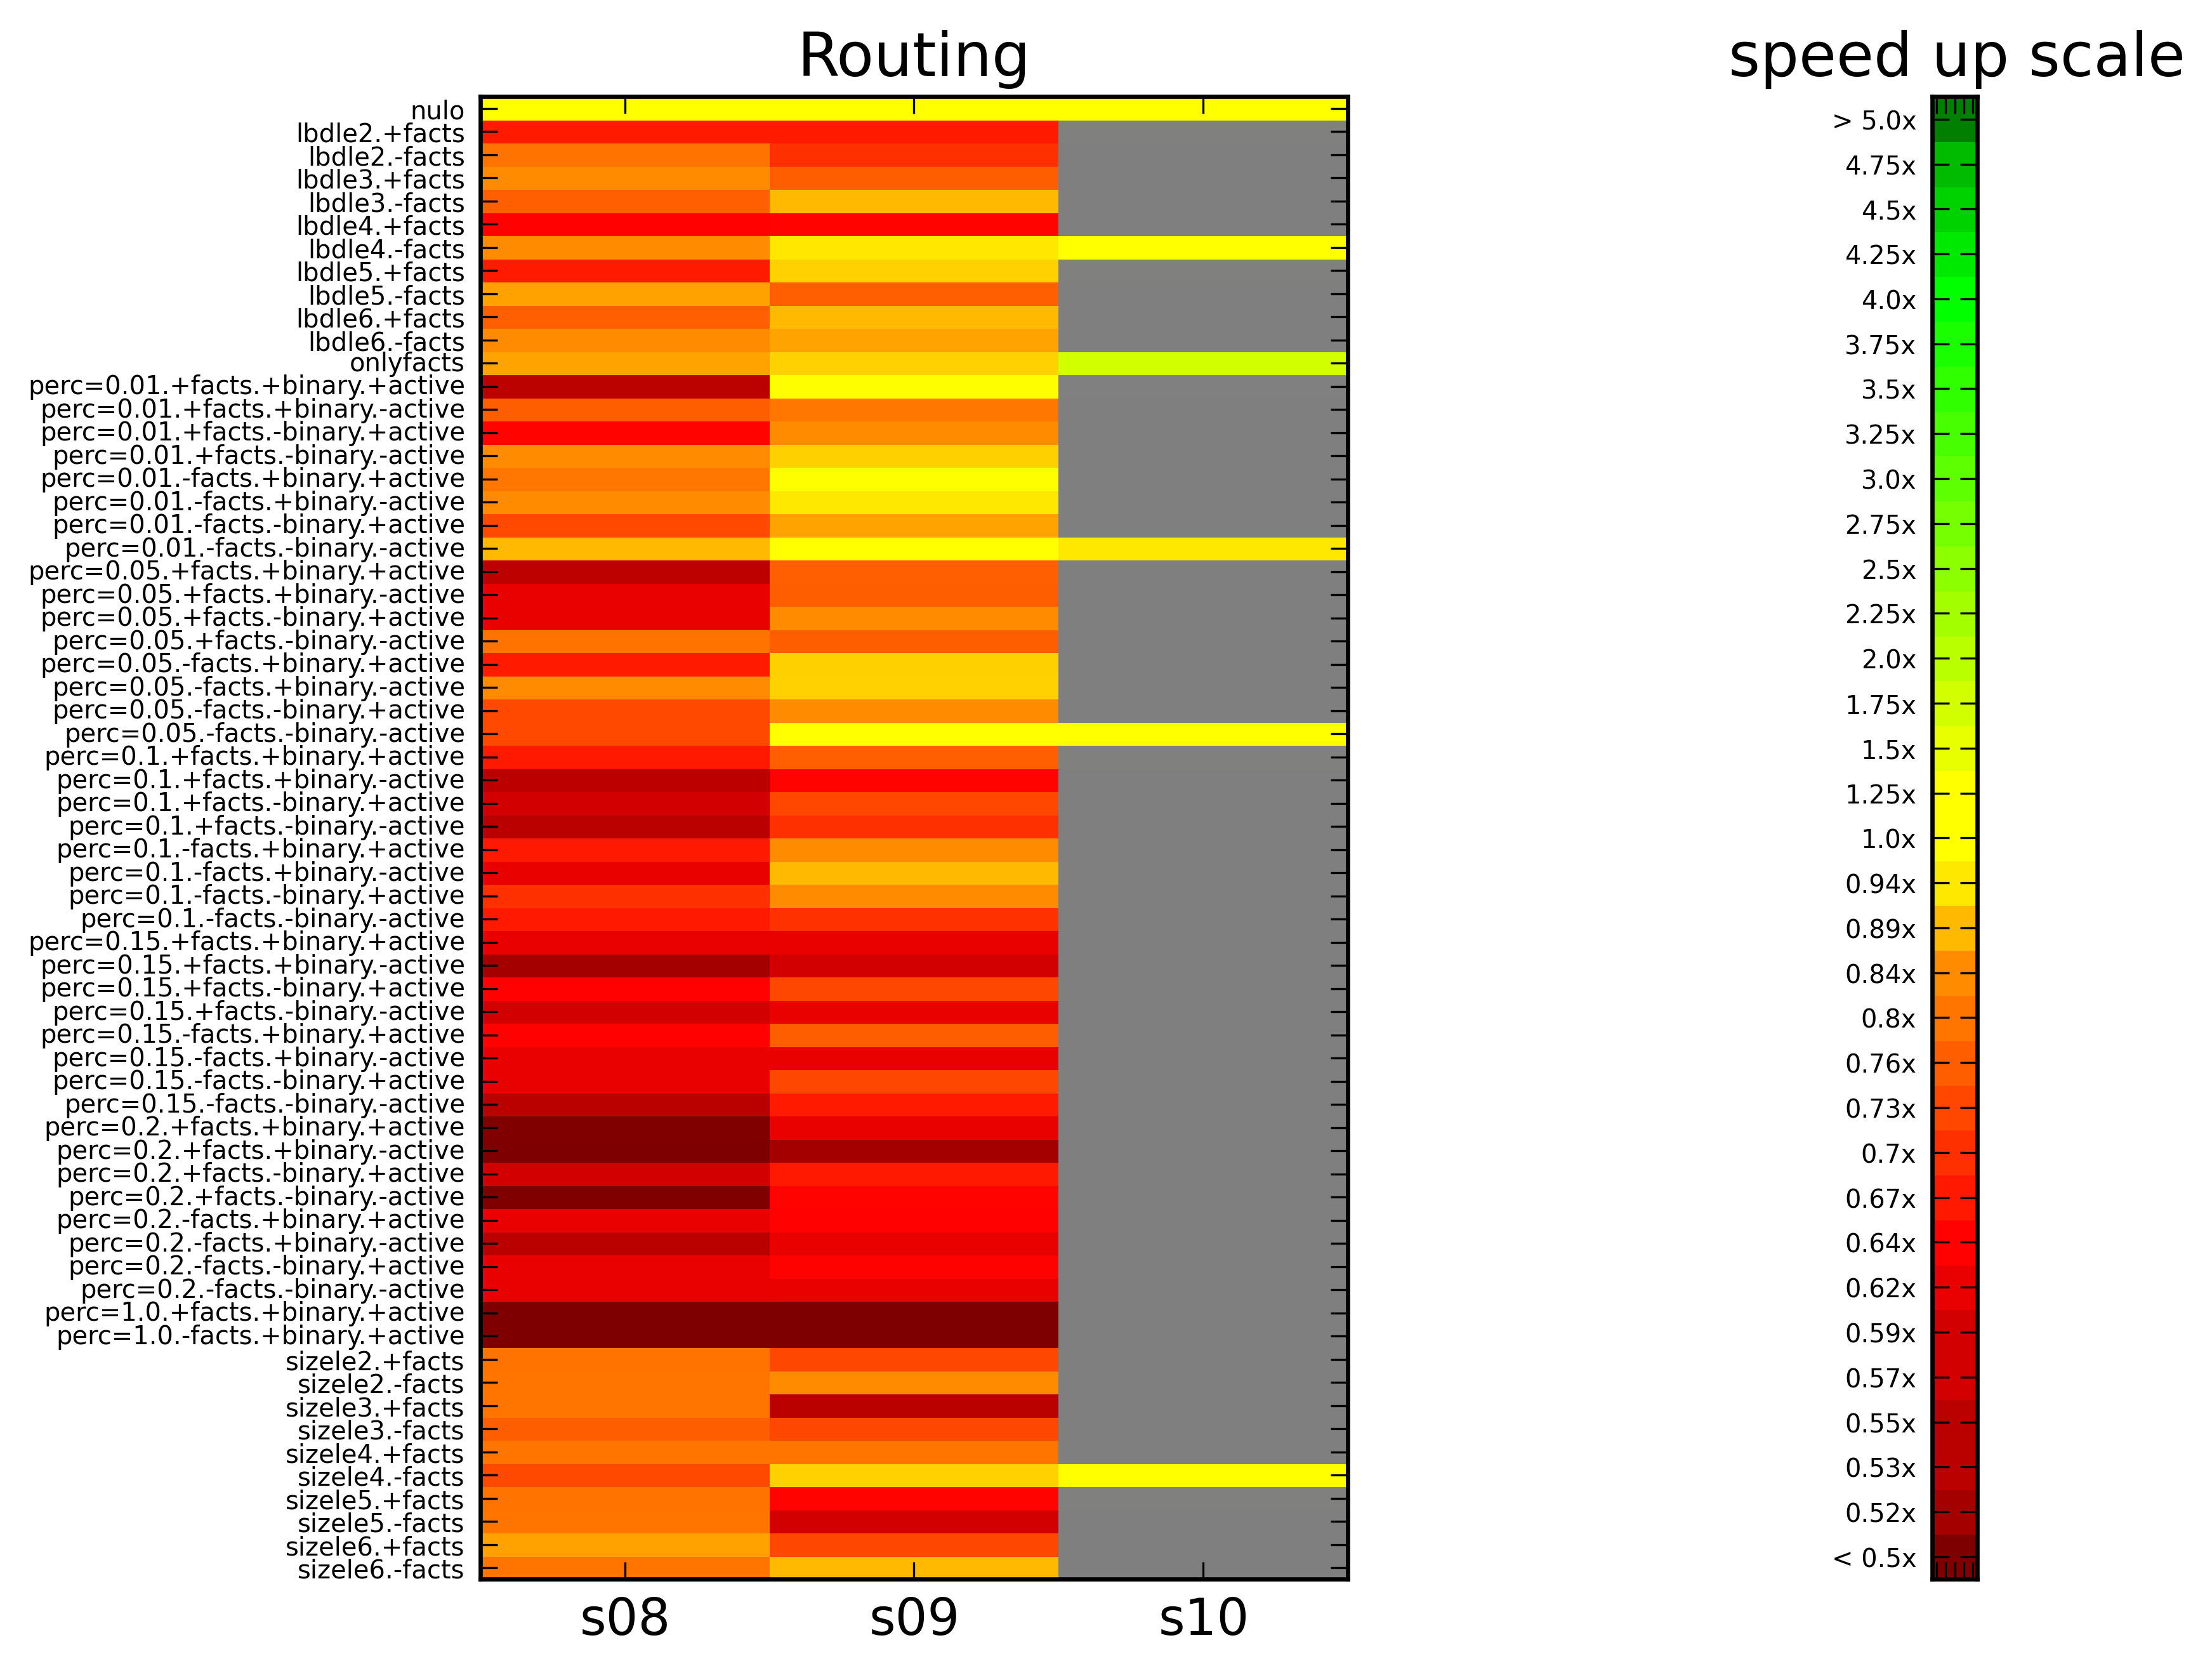
\includegraphics[width=\textwidth]{resultados/losp_heat.png}
	\caption{Comparación de criterios de herencia para distintos \emph{scopes} para el problema Routing}
	\label{res:learnscopespamela}
\end{figure}

\begin{figure}
	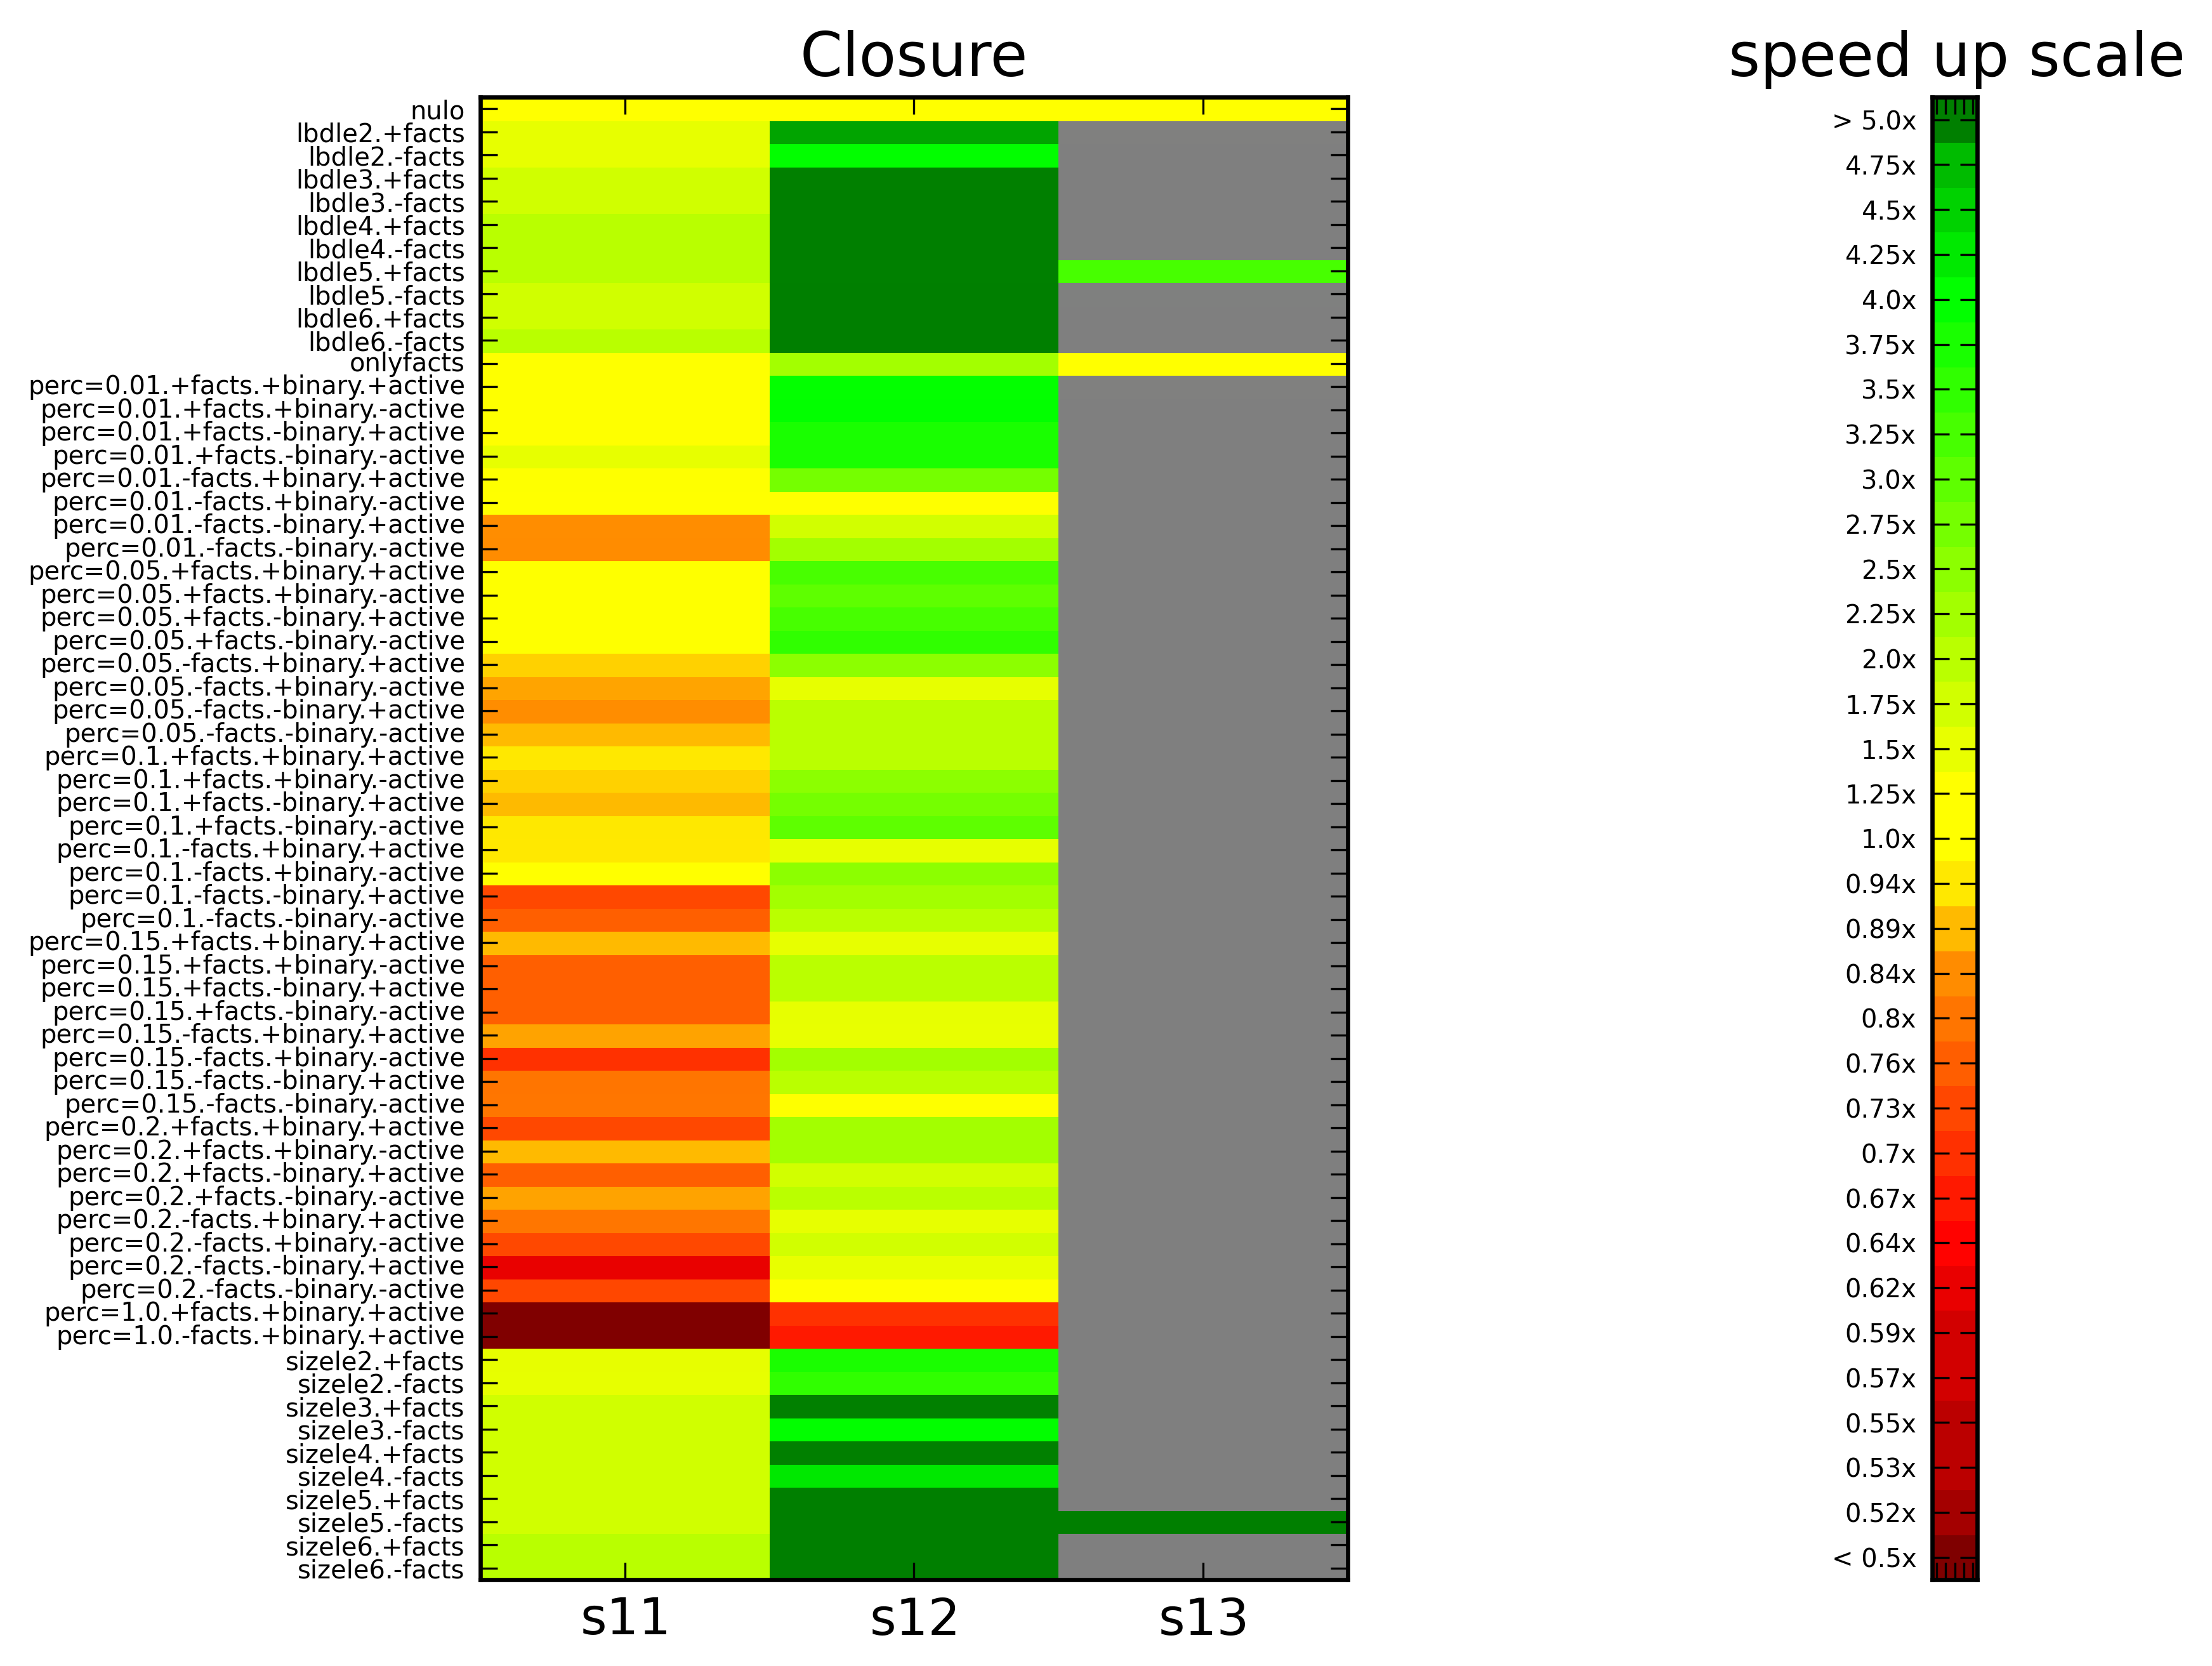
\includegraphics[width=\textwidth]{resultados/losk_heat.png}
	\caption{Comparación de criterios de herencia para distintos \emph{scopes} para el problema Closure}
	\label{res:learnscopesclosure}
\end{figure}

\begin{figure}
	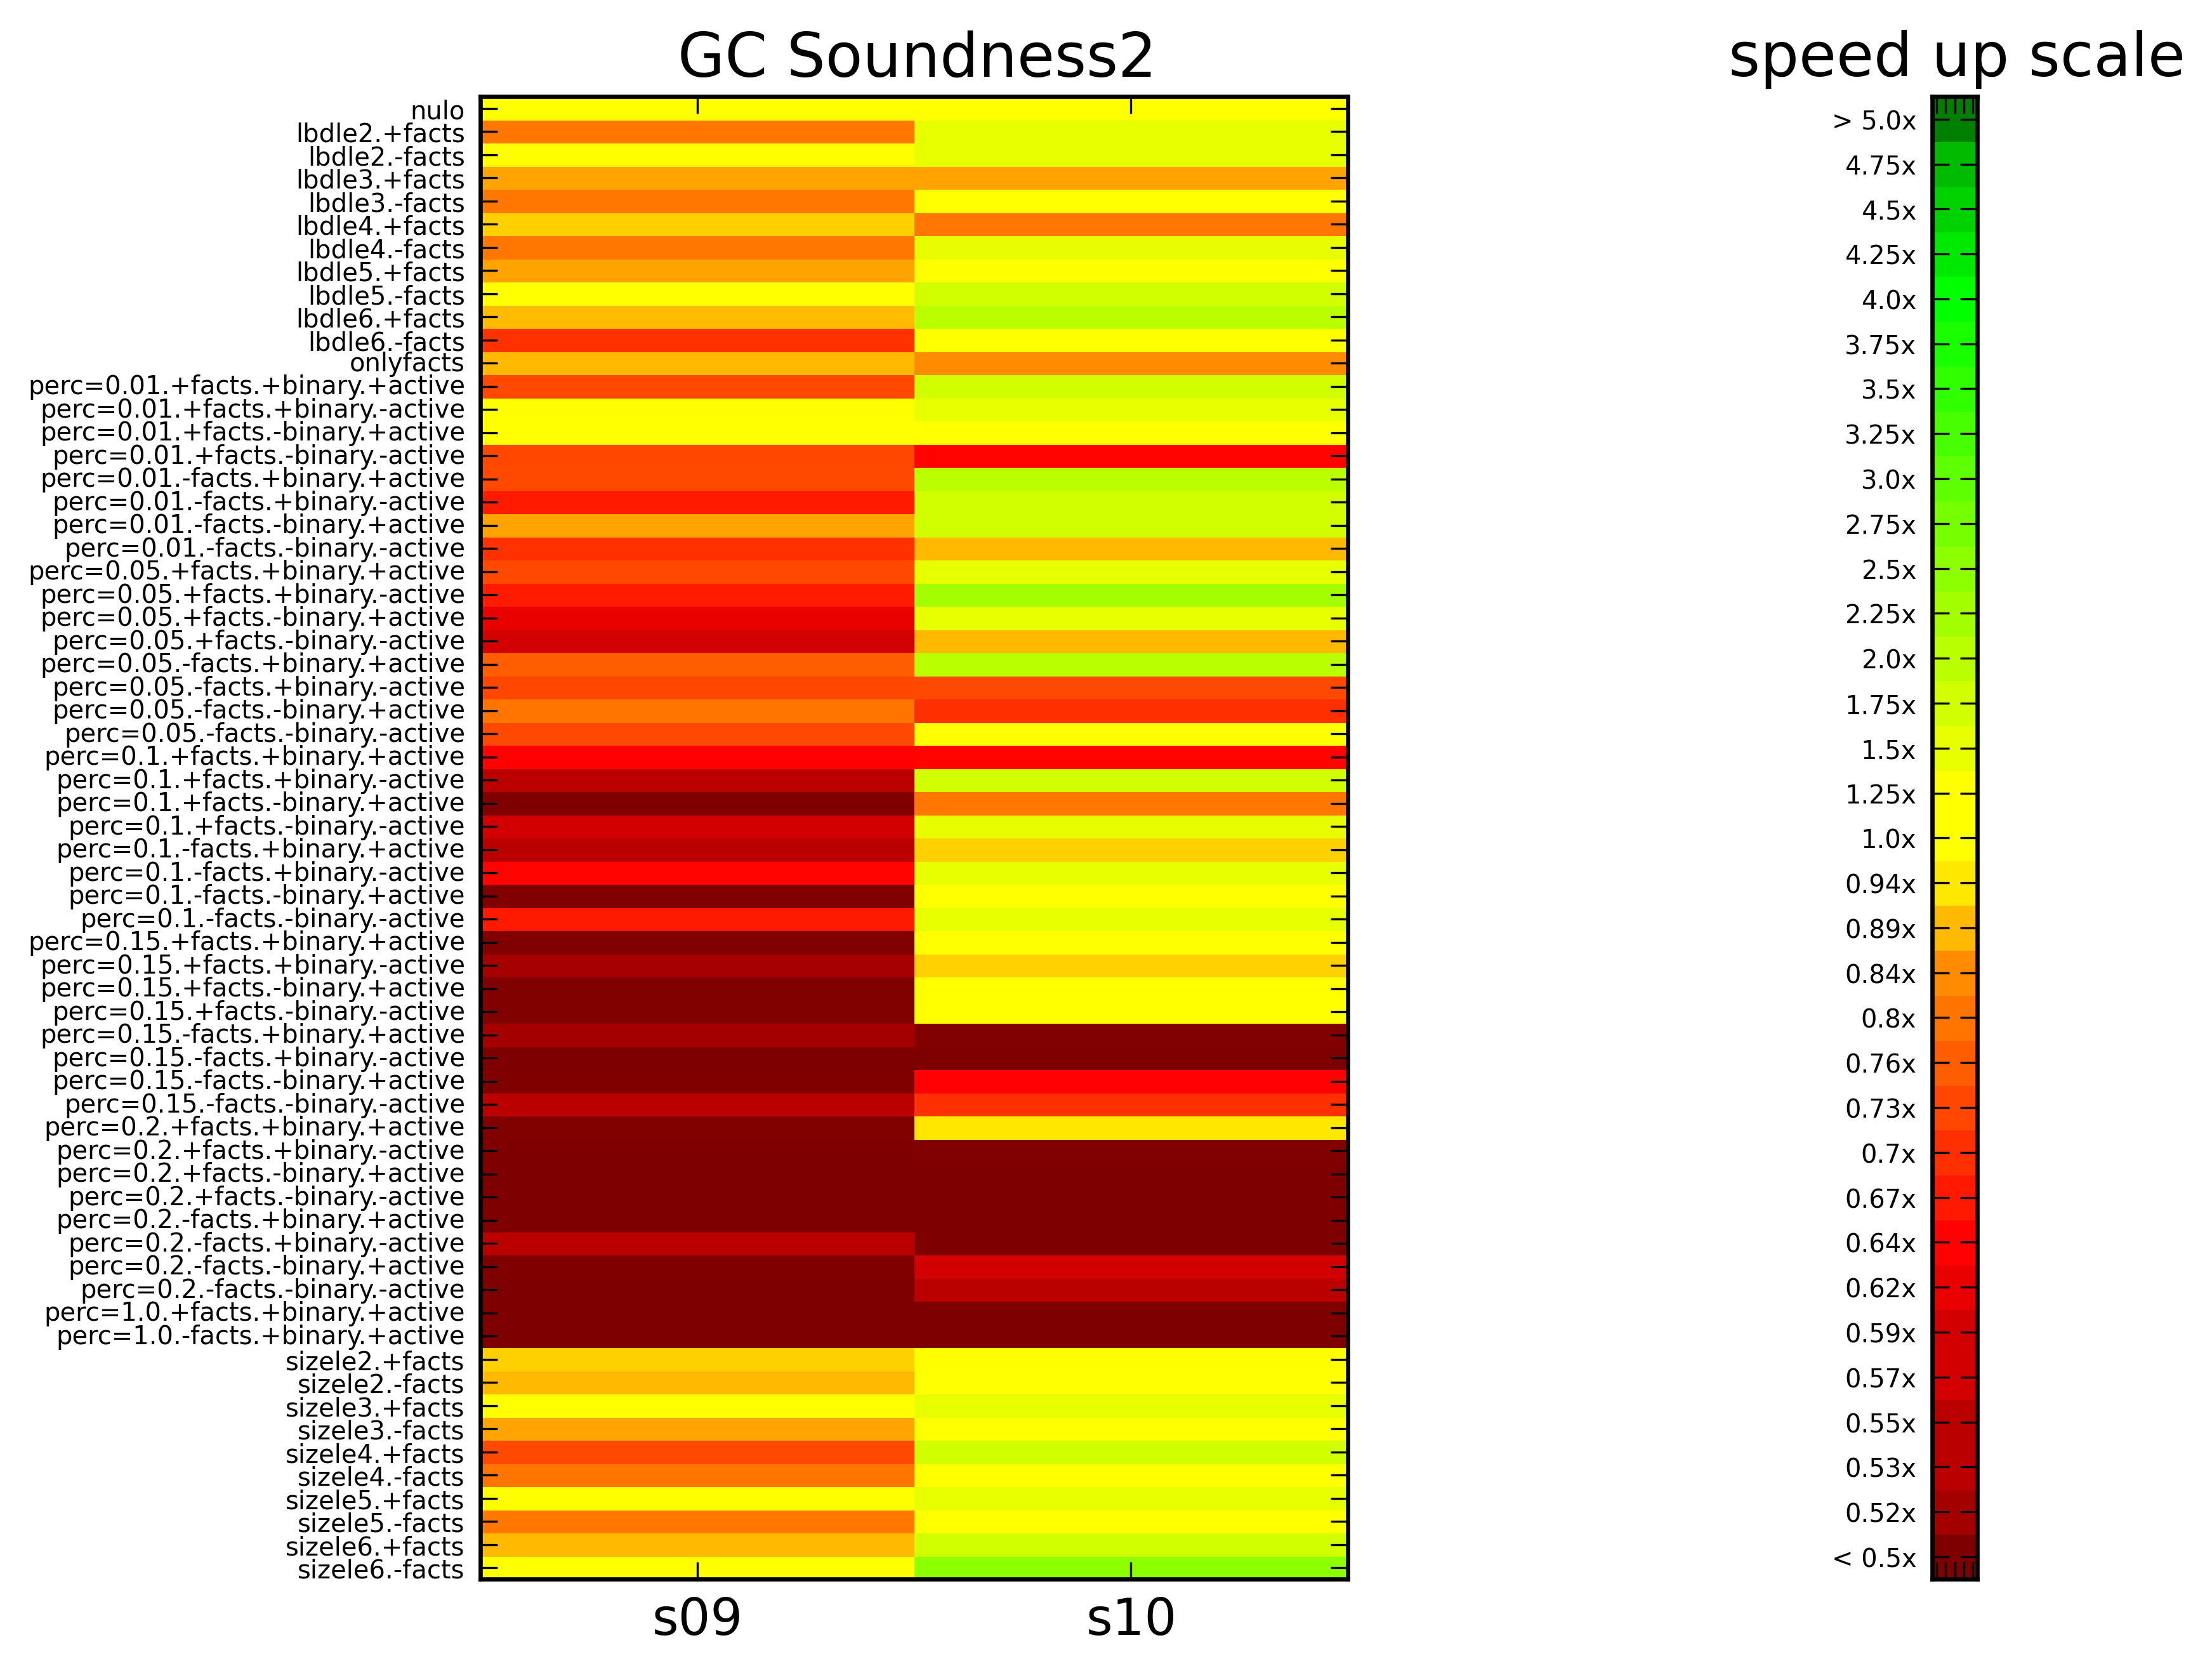
\includegraphics[width=\textwidth]{resultados/lossound_heat.png}
	\caption{Comparación de criterios de herencia para distintos \emph{scopes} para el problema GC Soundness2}
	\label{res:learnscopessoundness}
\end{figure}

\begin{figure}
	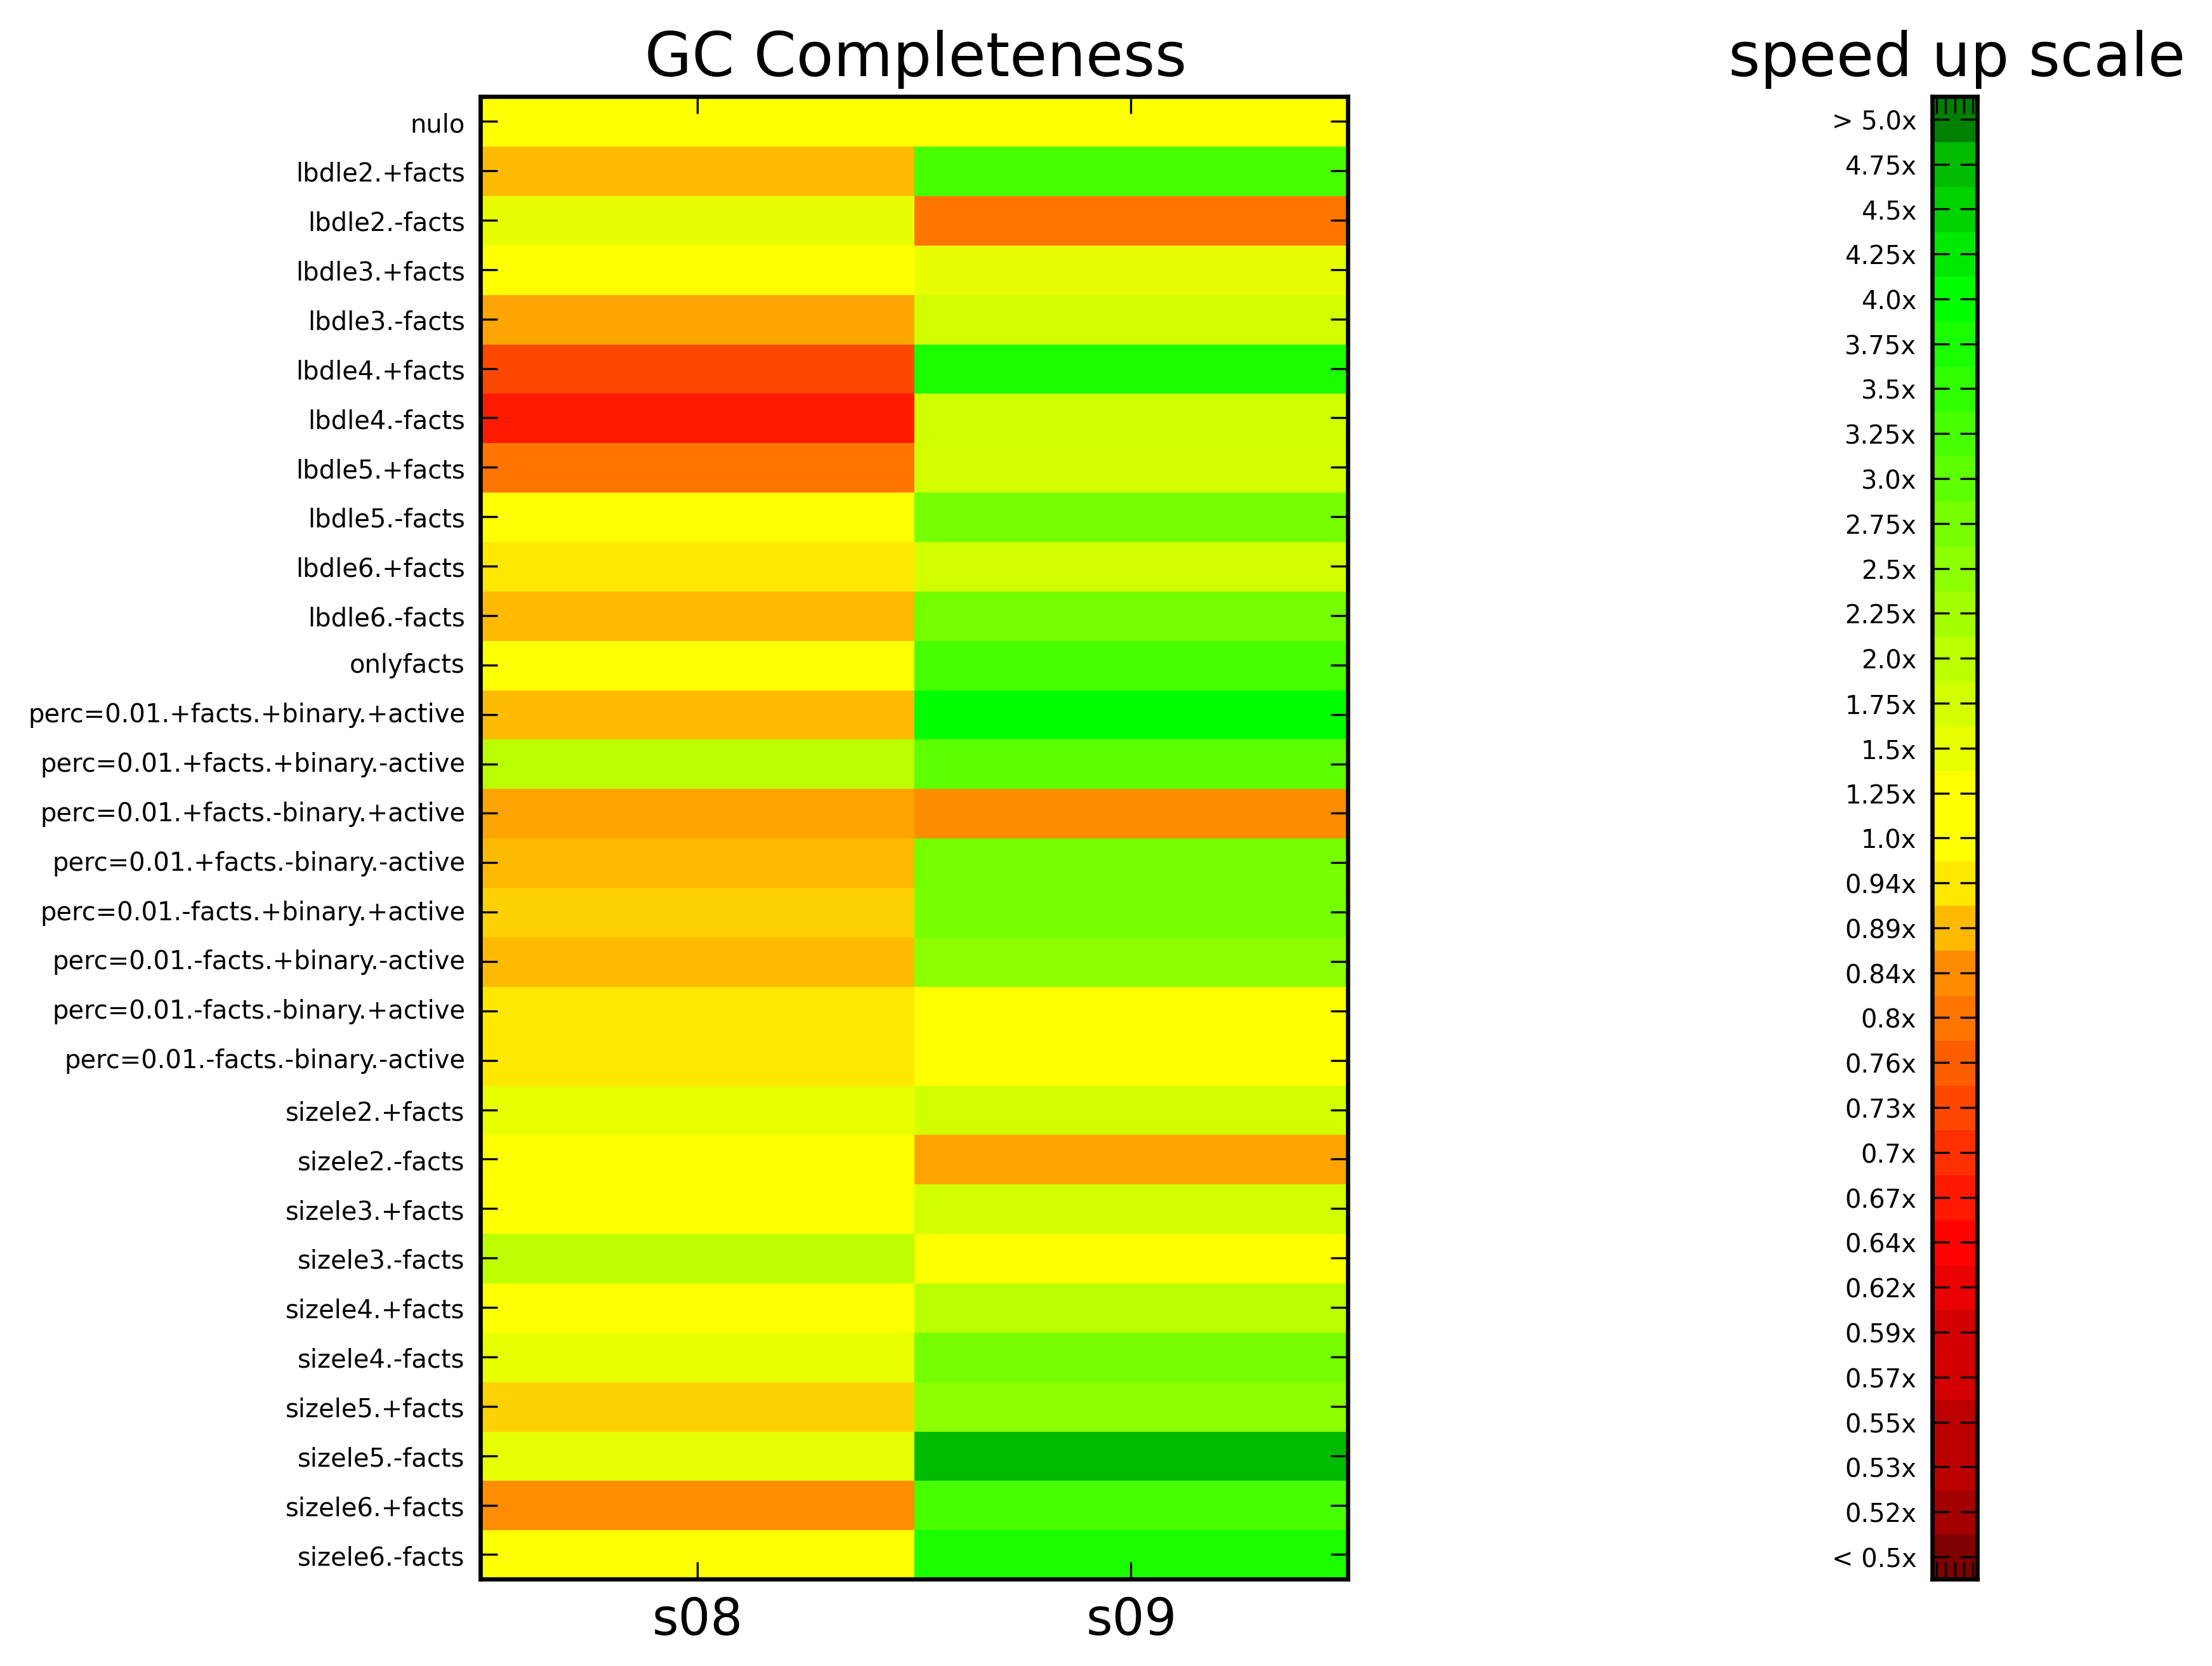
\includegraphics[width=\textwidth]{resultados/loscomp_heat.png}
	\caption{Comparación de criterios de herencia para distintos \emph{scopes} para el problema GC Completeness}
	\label{res:learnscopescompleteness}
\end{figure}

En primer lugar observamos que existe una tendencia a que, a medida que
aumenta el tamaño de un problema, la herencia de cláusulas obtiene mejores
resultados. Por un lado se ve que, criterios que en un \emph{scope}
presentaron resultados positivos, en el \emph{scope} siguiente presentan
resultados aún mejores. Del mismo modo los resultados negativos presentados
por algunos criterios se suavizan a medida que crece el \emph{scope} del
problema.

Consideramos que esto se debe a dos motivos. Por un lado existe un incremento
en los costos asociados a la generación, transmisión y carga de las tareas
cuando las mismas incluyen cláusulas aprendidas. Estos costos no crecen tan
rápidamente como el costo de análisis a medida que crece el \emph{scope}. Por
lo tanto el \emph{overhead} mencionado se va diluyendo a medida que el
problema requiere mayor tiempo de cómputo. Además, como ya hemos comentado en
la Sección~\ref{sec:pruning}, el uso de cláusulas aprendidas poda el espacio
de búsqueda al costo de ir en detrimento de la velocidad de propagación (BCP).
Así, su uso resulta particularmente necesario para resolver eficientemente
ciertos problemas grandes (donde el espacio de búsqueda se vuelve inmenso, y
cada poda es crucial para lograr agotarlo), pero a menudo es pernicioso para
los más chicos (donde el costo extra en cada propagación se vuelve
determinante).

También se observa que los resultados obtenidos por la herencia de cláusulas
varían considerablemente de problema en problema, pero a la vez se mantienen
coherentes a lo largo de los distintos \emph{scopes} de cada problema
particular. Como ejemplos paradigmáticos podemos destacar el problema Routing,
en el que la técnica tiende a no conseguir mejoras sustanciales aún en los
mejores casos, y el problema Closure, en el cual tiende a conseguir buenos
\emph{speedups} con la mayoría de los criterios. Esto sugiere la existencia de
cualidades intrínsecas a cada uno de los problemas que los hacen
inherentemente más (o menos) propensos a beneficiarse del enfoque propuesto.
Los experimentos realizados no son suficientes para aspirar a una extracción
de patrones comunes que permita aislar dichas cualidades.


Por último cabe destacar que, tal como intuíamos, el criterio que conserva la
totalidad de las cláusulas aprendidas por el padre resulta consistentemente
malo, tanto en términos absolutos (es siempre peor que no aprender nada) como
relativos (es siempre la peor alternativa). Además, observamos que existe un
subconjunto de los criterios probados que resulta consistentemente negativo.
Nos referimos a aquellos en los que se conserva el 10\% (o más) de las
cláusulas aprendidas por el padre. Es altamente probable que el mal desempeño
de estas alternativas se deba a las razones expuestas en la
Sección~\ref{sec:aboutcriteria}.

